\documentclass[xcolor=svgnames,11pt]{beamer}
% \documentclass[handout,xcolor=svgnames,11pt]{beamer}

\usepackage{graphicx}

\usepackage[english]{babel}
\usepackage[utf8x]{inputenc}
\usepackage[T1]{fontenc}
\usepackage[scale=0.9,sfdefault,light]{roboto}
\usepackage{hyperref}
\usepackage{tabularx}
\usepackage{url}
\usepackage{pbox}

\usepackage{etoolbox}
\makeatletter
\patchcmd{\insertverticalnavigation}%
{\ifx\beamer@nav@css\beamer@hidetext{\usebeamertemplate{section in sidebar}}\else{\usebeamertemplate{section in sidebar shaded}}\fi}%
{{\usebeamertemplate{section in sidebar}}}{}{}
\makeatother

\urlstyle{sf}

\usetheme{Goettingen}
\definecolor{leorange}{HTML}{FBA100}
\definecolor{leblue}{HTML}{003A70}
\definecolor{myblack}{RGB}{14,14,14}
\definecolor{lelightblue}{HTML}{BFCDDB}

\usecolortheme[named=leblue]{structure}
\beamertemplatenavigationsymbolsempty

\beamertemplateshadingbackground{white!15}{leorange!5}
\setbeamertemplate{sidebar canvas right}[vertical shading]%
[top=lelightblue,bottom=lelightblue]

\mode<presentation>{\usebackgroundtemplate{
\includegraphics
    [height=\paperheight]{img/back_le.png}}}

\setbeamertemplate{blocks}[rounded][shadow=false]
\setbeamercolor{block body}{bg=leorange!50}
\setbeamercolor{block title}{bg=leorange!80}

\setbeamercovered{transparent}

\title{\textbf{Let's Encrypt! Free certificates for everyone!}}
\author{Nicola Corti}
\institute{Gruppo Utenti Linux Pisa \\ \medskip 
\includegraphics[height=1.5cm]{img/gulp_logo.png}}
\logo{img/gulp_logo.png}
\date{03 February 2016}


\begin{document}

\begin{frame}
	\titlepage
\end{frame}

\section{Intro}
\begin{frame}{}
\begin{center}
\begin{Huge}
\textcolor{leorange}{\emph{Introduction}}
\end{Huge}
\end{center}
\end{frame}



\begin{frame}{What is Let's Encrypt?}
\begin{center}

\includegraphics[width=5cm]{img/logo_le.png}
\end{center}

\begin{block}{}
Let's Encrypt is a \textbf{Certification Authority (CA)} that issue \textbf{free} SSL/TLS certificates
\end{block}
\pause \medskip
\begin{itemize}
  \item From 5 December 2015 L.E. is available in \textbf{Public Beta}
  \pause
  \item L.E. has released more than \textbf{480 k} certificates
  \pause
  \item It's major focus is \textbf{automation} of processes.
  \pause
  \item \textbf{\url{https://letsencrypt.org/}}
\end{itemize}
\end{frame}

\subsection{Sponsors}
\begin{frame}{Sponsors}
\begin{center}
Who's behind the project?
\medskip
\vspace{0.5cm}
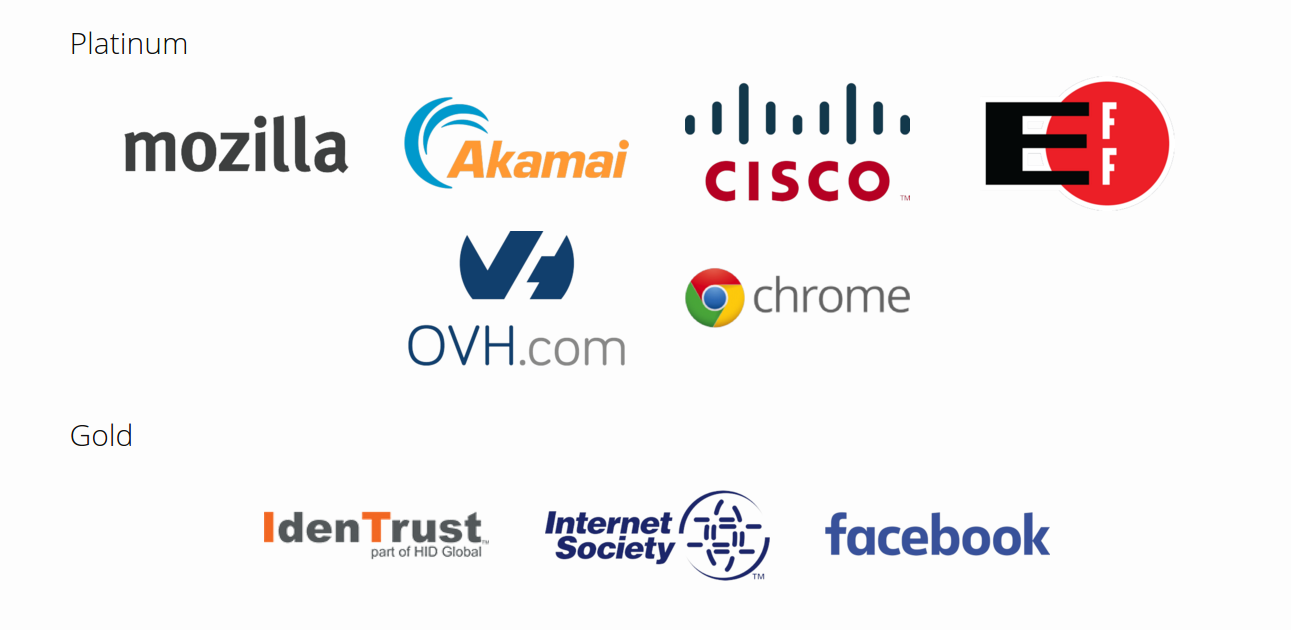
\includegraphics[width=10cm]{img/sponsors.png}
\end{center}
\end{frame}

\subsection{History}
\begin{frame}{History}
\begin{description}
  \item[2012] Project begins inside \textbf{Mozilla}
  \pause
  \item[11-2014] Let's Encrypt \textbf{publicly announced}
  \pause
  \item[01-2015] The \textbf{ACME} protocol submitted to \textbf{IETF} for standardization
  \pause
  \item[04-2015] \textbf{ISRG} (Internet Security Research Group) and \textbf{Linux Foundation} join the project
  \pause
  \item[09-2015] Issued the first certificate for \textbf{\href{https://helloworld.letsencrypt.org/}{helloworld.letsencrypt.org}}
  \pause
  \item[10-2015] L.E. intermediate certificate becomes \textbf{\emph{cross-signed}} by IdenTrust.
  (\emph{Let's Encrypt is trusted!})
  \pause
  \item[12-2015] \textbf{Public beta!}
\end{description}
\end{frame}

\subsection{Why?}
\begin{frame}{Why?}
\begin{itemize}
  \item \textbf{Free}
  \medskip\pause
  \item \textbf{Automated}
  \medskip\pause
  \item \textbf{Open}
  \medskip\pause
  \item \textbf{Secure}
  \medskip\pause
  \item \textbf{Transparent}
\end{itemize}
\end{frame}

\section{Server}
\begin{frame}{}
\begin{center}
\begin{Huge}
\textcolor{leorange}{\emph{Server}}
\end{Huge}
\end{center}
\end{frame}



\begin{frame}{Boulder}
\begin{block}{Architecture}
The Let's Encrypt system is based on \textbf{3 components}: a \textbf{server}, a \textbf{client} and the \textbf{protocol} that defines the communication rules between server and client
\end{block}

\medskip \pause

The server is called \textbf{Boulder} and it's completely written in \textbf{Go}. It's responsible of handling all the procedures for \textbf{issuing}, \textbf{renewal} and \textbf{revocation} of certificates.
\medskip \pause

It's basically an HTTPS server that exposes a \textbf{RESTful} interface.

\medskip \pause

\begin{center}
\visible<4>{
\includegraphics[width=0.3cm]{img/logo_gh.pdf}} \textbf{\url{https://github.com/letsencrypt/boulder}}
\end{center}
\end{frame}

\section{Client}
\begin{frame}{}
\begin{center}
\begin{Huge}
\textcolor{leorange}{\emph{Client}}
\end{Huge}
\end{center}
\end{frame}

\begin{frame}{letsencrypt}
The client is called (obviously) \textbf{letsencrypt} and it's completely written in \textbf{Python}.
It's responsible for interaction with the remote server and it \textbf{handles your certificates}.
\pause
\begin{itemize}
  \item Download through .deb package \textbf{letsencrypt} (only on debian \emph{sid/stretch}).
  \item Clone the \textbf{git repository}.
\end{itemize}
\pause
\begin{center}
\visible<3>{
\includegraphics[width=0.3cm]{img/logo_gh.pdf}} \textbf{\url{https://github.com/letsencrypt/letsencrypt}}
\end{center}
\end{frame}

\begin{frame}{Plugins}
The client's main purpose is to \textbf{simplify and automate}
the whole process of authentication and creation of the certificate.

\medskip\pause

For this reason the client comes with several plugins, useful to automatically setup the new certificates on popular web servers:
\textbf{apache} and \textbf{nginx}.

\visible<2>{
\begin{center}

\includegraphics[height=2cm]{img/apache_logo.png}

\includegraphics[height=2cm]{img/nginx_logo.png}
\end{center}}

\end{frame}

\section{Protocol}
\begin{frame}{}
\begin{center}
\begin{Huge}
\textcolor{leorange}{\emph{Protocol}}
\end{Huge}
\end{center}
\end{frame}


\begin{frame}{ACME}

\begin{block}{}
The procol use by Let's Encrypt is called \textbf{Automated Certificate Management Environment (ACME)}.
\end{block}

\medskip \pause
ACME is based on exchanges of signed \textbf{JSON} files (a.k.a. \textbf{JWS, Json Web Signature}).
These documents contains all the requests and the responses between the client and the server.

\medskip \pause
These documents \textbf{must} be exchanged over \textbf{HTTPS}.
\end{frame}

\begin{frame}{ACME}
\begin{center}
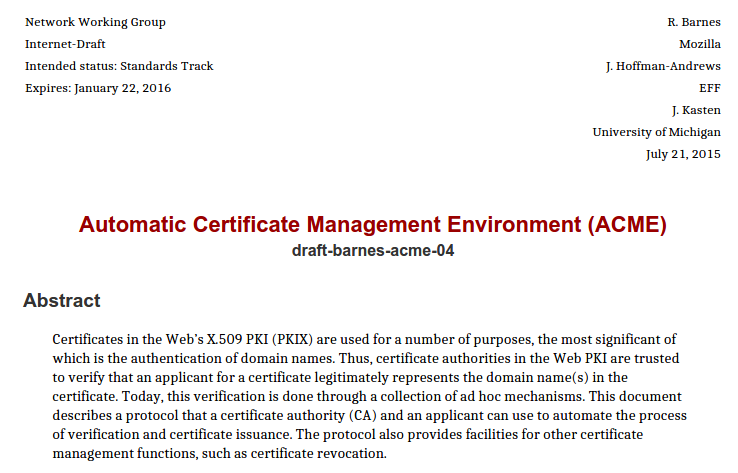
\includegraphics[width=9.5cm]{img/acme_spec.png}


\includegraphics[width=0.3cm]{img/logo_gh.pdf} \textbf{ \url{https://github.com/letsencrypt/acme-spec}}
\end{center}
\end{frame}


\begin{frame}{ACME}
The ACME protocol is aimed to:
\pause\medskip
\begin{enumerate}
  \item \textbf{Prove} that we are the owners of a specific domain, say \emph{example.com}
  \pause\medskip
  \item \textbf{Obtain} a new certificate for the domain \emph{example.com}
  \pause\medskip
  \item \textbf{Revoke} or \textbf{Renew} a certificate for the domain \emph{example.com}
\end{enumerate}
\end{frame}

\subsection{Security}
\begin{frame}{Security}
All the interactions between client and servers are encrypted with a \textbf{public/private key pair} generated during the first execution of the client.

\medskip \pause

\begin{block}{}
In order to \textbf{prove} that we are the owners of the domain, the server sends us a set of \textbf{challenges} that we must solve.
\end{block}

\medskip \pause

Every interaction with the server is marked with a \textbf{nonce} number that allows to avoid \textbf{Replay} attacks.

\end{frame}

\subsection{Challenges}
\begin{frame}[fragile]{Challenges}
\begin{center}

The server can decide to send one or more challenge from the followings:
\medskip\pause

\begin{tabular}{p{3cm}p{6cm}}

\hline
\textbf{Type} & \textbf{Description} \\
\hline
\textcolor{leblue}{\textbf{\small Simple HTTP}} & \textcolor{leblue}{\small 
You must place a \textbf{token file} inside your webserver root folder.
Both HTTP and HTTPS are accepted} \\
\hline
\textbf{\small DNS} & {\small You must provide a token inside a \textbf{TXT record} of your DNS server} \\
\hline\hline
\textbf{\scriptsize Proof of possession} & {\scriptsize You must \textbf{sign a document} using a keypair that the server already consider yours} \\
\hline
\textbf{\scriptsize Domain Validation with Server Name Indication} & {\scriptsize You must configure a \textbf{TLS server} on a specific IP address (through an A record inside the DNS).} \\
\hline
\end{tabular}
\end{center}
\end{frame}

\subsection{The protocol}
\begin{frame}{Domain Validation}
\begin{center}
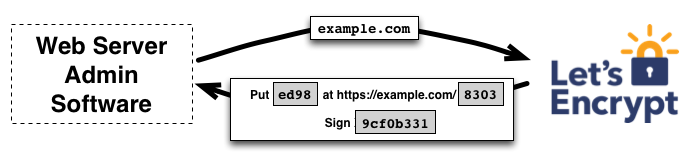
\includegraphics[width=9cm]{img/proto_1.png}
\end{center}
\end{frame}

\begin{frame}{Domain Validation}
\begin{center}
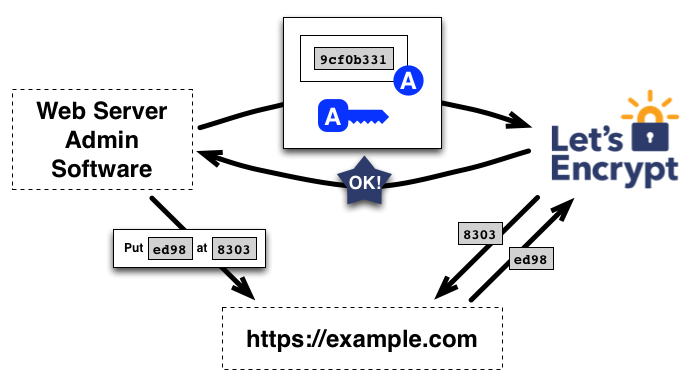
\includegraphics[width=9cm]{img/proto_2.png}
\end{center}
\end{frame}

\begin{frame}{Certificate Issuance}
\begin{center}
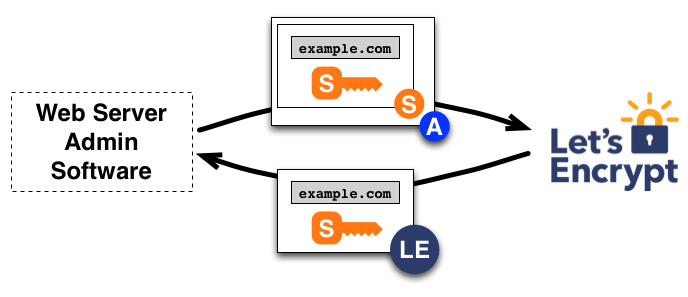
\includegraphics[width=9cm]{img/proto_3.png}
\end{center}
\end{frame}

\subsection{Cert revocation}
\begin{frame}{Certificate Revocation}
\begin{center}
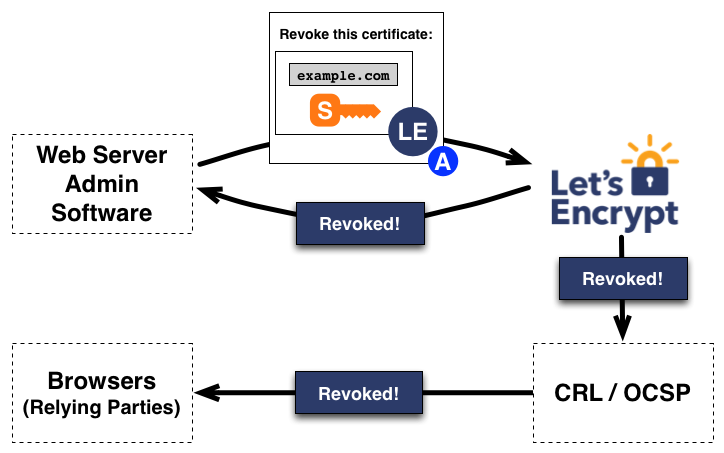
\includegraphics[width=9cm]{img/proto_4.png}
\end{center}
\end{frame}

\section{Certs}
\begin{frame}{}
\begin{center}
\begin{Huge}
\textcolor{leorange}{\emph{Certificates}}
\end{Huge}
\end{center}
\end{frame}


\subsection{DV}
\begin{frame}{DV Certificates}
\begin{block}{DV}
All the certificates issue from L.E. are \textbf{Domain Validated} certificates. They basically prove that you are the owner of a specific domain, nothing more.
\end{block}
\medskip\pause

\textbf{Organization Validation} and \textbf{Extended Validation} certificates 
requires to explicit verify the identity of the subject that is requesting a certificate.

\visible<2>{
\begin{center}
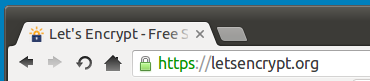
\includegraphics[width=6cm]{img/dv_example.png}

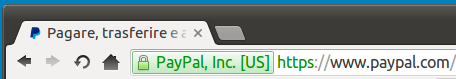
\includegraphics[width=6cm]{img/ev_example.png}
\end{center}}
\end{frame}

\subsection{Cross Signing}
\begin{frame}{Cross Signing}
All the issued certificates are \emph{Cross-signed} by \textbf{IdenTrust}.
In this way, all the L.E. certificates are trusted by major browsers.

\medskip\pause

We can avoid browser errors such as:

\visible<2>{
\begin{center}
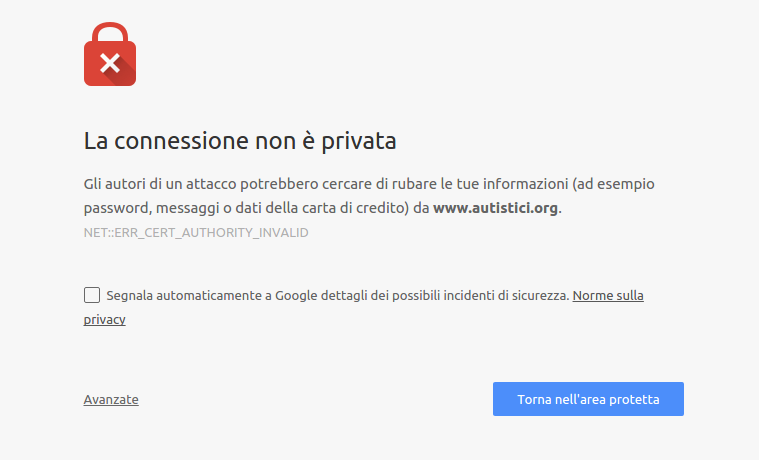
\includegraphics[width=7cm]{img/cert_error.png}
\end{center}}
\end{frame}

\begin{frame}{Cross Signing}
\begin{center}
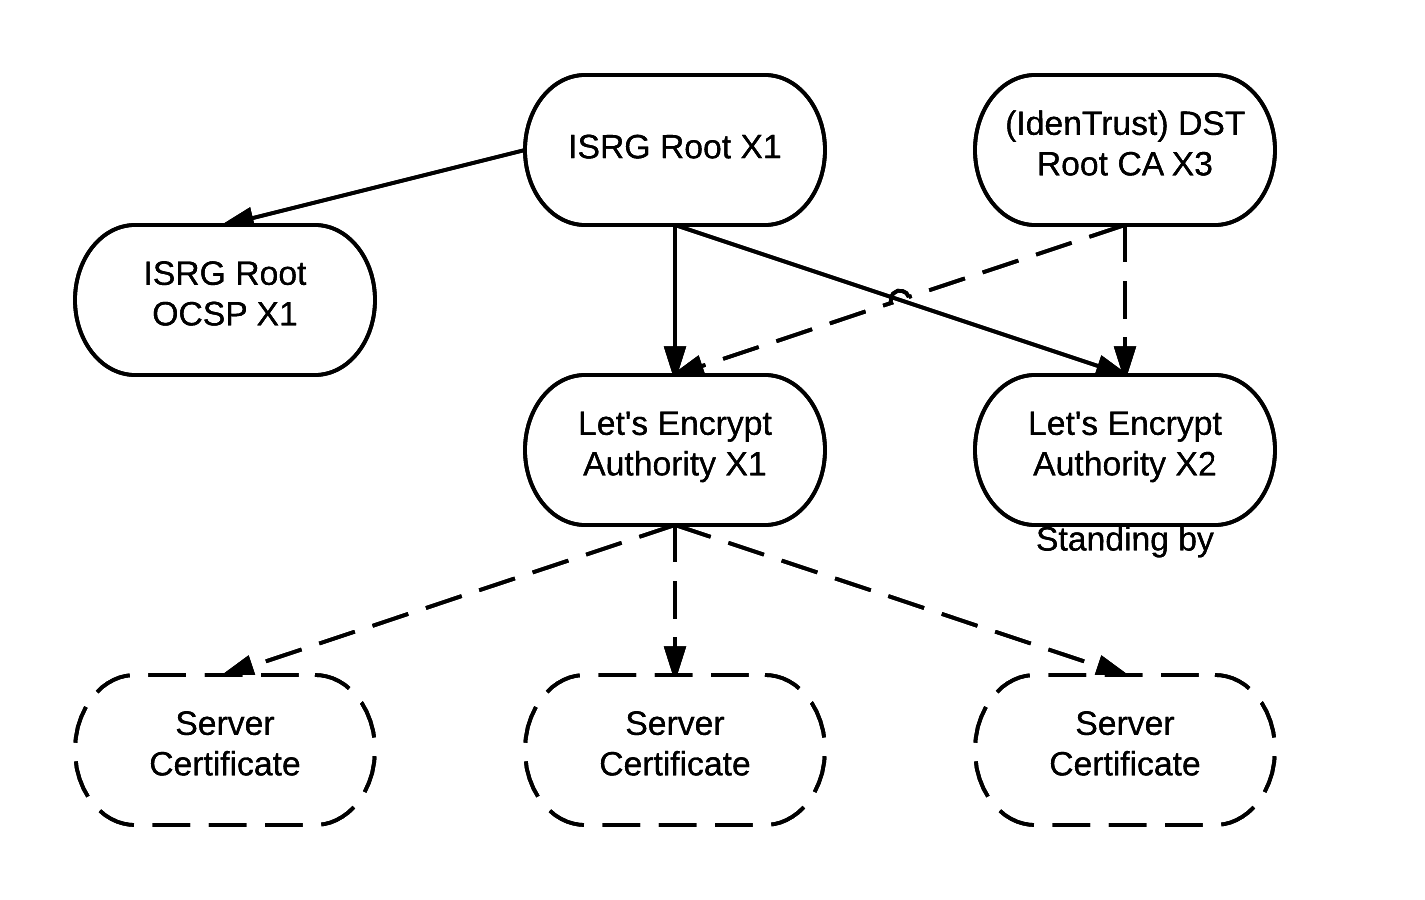
\includegraphics[width=10cm]{img/certs.png}
\end{center}
\end{frame}

\begin{frame}{Validity}
All the certificates have a \textbf{90 days} validity. After the expiry, the certificates are not valid anymore and the browsers will raise security errors.

\medskip\pause

\begin{block}{\emph{90-days validity}}
This is nothing new on the web. Having certificates with a reduced validity could help to limit damage from key compromise and mis-issuance.
\end{block}

\medskip\pause
You will receive \emph{remind emails} whenever a certificate is near to expire. Certificate renewal can be automated with a \textbf{cron} task.
\end{frame}


\section{Setup}
\begin{frame}{}
\begin{center}
\begin{Huge}
\textcolor{leorange}{\emph{Setup}}
\end{Huge}
\end{center}
\end{frame}


\subsection{Requirements}
\begin{frame}{Requirements}
The client minimal requirements are: 
\begin{itemize}
  \item \textbf{Unix like} system.
  \item \textbf{Python 2.6} or \textbf{2.7}.
  \item \textbf{root} rights on the system.
\end{itemize}

\medskip\pause

The \textbf{apache} setup plugins works only on Debian based system: \textbf{Ubuntu 12.04+} and \textbf{Debian 7+}
\end{frame}

\subsection{Download}
\begin{frame}[fragile]{Download}
First, let's download the \textbf{letsencrypt} client.

\medskip\pause
On Debian \emph{sid/stretch}:
\begin{block}{}
\begin{scriptsize}
\begin{verbatim}
$ sudo apt-get install letsencrypt
$ letsencrypt --help
\end{verbatim}
\end{scriptsize}
\end{block}

\medskip\pause
On other OS:
\begin{block}{}
\begin{scriptsize}
\begin{verbatim}
$ git clone https://github.com/letsencrypt/letsencrypt
$ cd letsencrypt
$ ./letsencrypt-auto --help
\end{verbatim}
\end{scriptsize}
\end{block}

\medskip\pause

From now on we will use \textbf{letsencrypt-auto} for all the commands, assuming to proceed with clone of the repository.

\end{frame}

\subsection{Run}
\begin{frame}[fragile]{Run}
To execute the client you simply have to invoke:
\begin{block}{}
\begin{scriptsize}
\begin{verbatim}
$ ./letsencrypt-auto
\end{verbatim}
\end{scriptsize}
\end{block}
We will be guided through the issuing process
\end{frame}

\begin{frame}[fragile]{Apache}
If you want to automatically configure \textbf{Apache} with the generated certificates you can invoke:
\begin{block}{}
\begin{scriptsize}
\begin{verbatim}
$ ./letsencrypt-auto --apache -d example.com -d www.example.com
\end{verbatim}
\end{scriptsize}
\end{block}
With \textbf{-{}-apache} we are enabling the apache plugin, and with \textbf{-d} we are giving the list of involved domains.
\end{frame}

\begin{frame}[fragile]{Contacts}
During the first run, the client will ask for our \textbf{mail address}
and it will request to accept the \textbf{Terms of service}.

\medskip\pause

You can skip these steps using these flags:

\medskip

\begin{block}{}
\begin{scriptsize}
\begin{verbatim}
$ ./letsencrypt-auto --email admin@example.com --agree-tos
\end{verbatim}
\end{scriptsize}
\end{block}
\end{frame}

\subsection{Plugins}
\begin{frame}{Plugins}
\begin{center}
\begin{tabular}{p{2cm}p{0.5cm}p{0.5cm}p{5cm}}
\hline
\textbf{Plugin} & \textbf{A} & \textbf{I} & \textbf{Descrizione}\\
\hline
Apache & Y & Y & {\scriptsize Obtain and setup automatically the certs. on Apache 2.4 (Debian based)} \\
Standalone & Y & N & {\scriptsize Obtain the cert with a \textbf{standalone} web server on ports 80/443} \\
Webroot & Y & N & {\scriptsize Obtain a certificate \emph{touching} a token inside the root folder of an already existing webserver}\\
Manual & Y & N & {\scriptsize Prints the commands to manually obtain the certs from a different client} \\
Nginx & Y & Y & {\scriptsize Obtain and setup automatically the certs. on nginx (experimental)} \\
\hline
\end{tabular}
\end{center}
\end{frame}


\begin{frame}[fragile]{certonly}
You can use the plugins with \textbf{authentication} support (A column) just to obtain the certificates \textbf{without installation}.

\medskip\pause

Simply add the option \textbf{certonly} to the command line.

\medskip

\begin{block}{Standalone example}

\begin{scriptsize}
\begin{verbatim}
$ ./letsencrypt-auto --standalone-supported-challenges \
 http-01 certonly -d example.com
\end{verbatim}
\end{scriptsize}

This command will start a standalone webserver on port 80 and it will obtain the certificate for example.com
\end{block}
\end{frame}

\begin{frame}{/etc/letsencrypt}
All the certificates and the auth keys will be saved into
\textbf{/etc/letsencrypt}.

\medskip\pause
{
\setbeamercolor{block body}{bg=red!50}
\begin{block}{}
Inside this folder you will find all the \textbf{certificates} and all the \textbf{public/private keys}.
It's \textbf{extremely} recommended to make a \textbf{backup} of this folder to a secure place.
\end{block}
}
\medskip\pause
Inside \textbf{/etc/letsencrypt/live/example.com/} you will find symlinks that will be updated after every renewal.
\end{frame}

\begin{frame}{/etc/letsencrypt}
You will find the following files:
\begin{description}
  \item[\textbf{\small privkey.pem}] Private key of the certificate. DO NOT SHARE IT!
  \item[\textbf{\small cert.pem}] Webserver certificate (sent to the browser).
  \item[\textbf{\small chain.pem}] List of all the intermediate certificates connected to this certificate.
  \item[\textbf{\small fullchain.pem}] cert.pem + chain.pem
\end{description}
\end{frame}

\subsection{Revoke}
\begin{frame}[fragile]{Revoke}
To revoke a certificate you can simply use the option \textbf{revoke}.

\medskip\pause

\begin{block}{}
\begin{scriptsize}
\begin{verbatim}
$ /.letsencrypt-auto revoke --cert-path example-cert.pem
\end{verbatim}
\end{scriptsize}
\end{block}
\end{frame}

\subsection{Renewal}
\begin{frame}[fragile]{Renewal}
The renewal process it's extremely easy, you can simply invoke \textbf{letsencrypt} without parameters.

\medskip\pause

You can also use the \textbf{-{}-renew-by-default} to perform the automatic renewal of the certificate without user interaction.

\medskip\pause

In this way, it's possible to schedule a \textbf{cron} task to automatically renew the certificates before the expiry.

\end{frame}

\subsection{Update}
\begin{frame}[fragile]{Update}
Since Let's Encrypt it's a public beta, it's fundamental to keep the client up to date.

\medskip\pause
On Debian \emph{sid/stretch}:
\begin{block}{}
\begin{scriptsize}
\begin{verbatim}
$ apt-get update && apt-get upgrade
\end{verbatim}
\end{scriptsize}
\end{block}

\medskip\pause
On other OS:
\begin{block}{}
\begin{scriptsize}
\begin{verbatim}
$ cd letsencrypt
$ git pull
\end{verbatim}
\end{scriptsize}
\end{block}

\end{frame}

\begin{frame}[fragile]{General usage}
During everyday usage, you can simply invoke letsencrypt without parameters. The \emph{terminal UI} will guide you through the desidered process.

\medskip\pause

You simply have to answer to the client questions.

\medskip\pause

Having only \textbf{too much parameters} could be hard to remember. The UI will help on this, but the parameter still give the flexibility to embed the client inside \textbf{scripts}.

\end{frame}

\subsection{Screens}
\begin{frame}{Screens}
\begin{center}
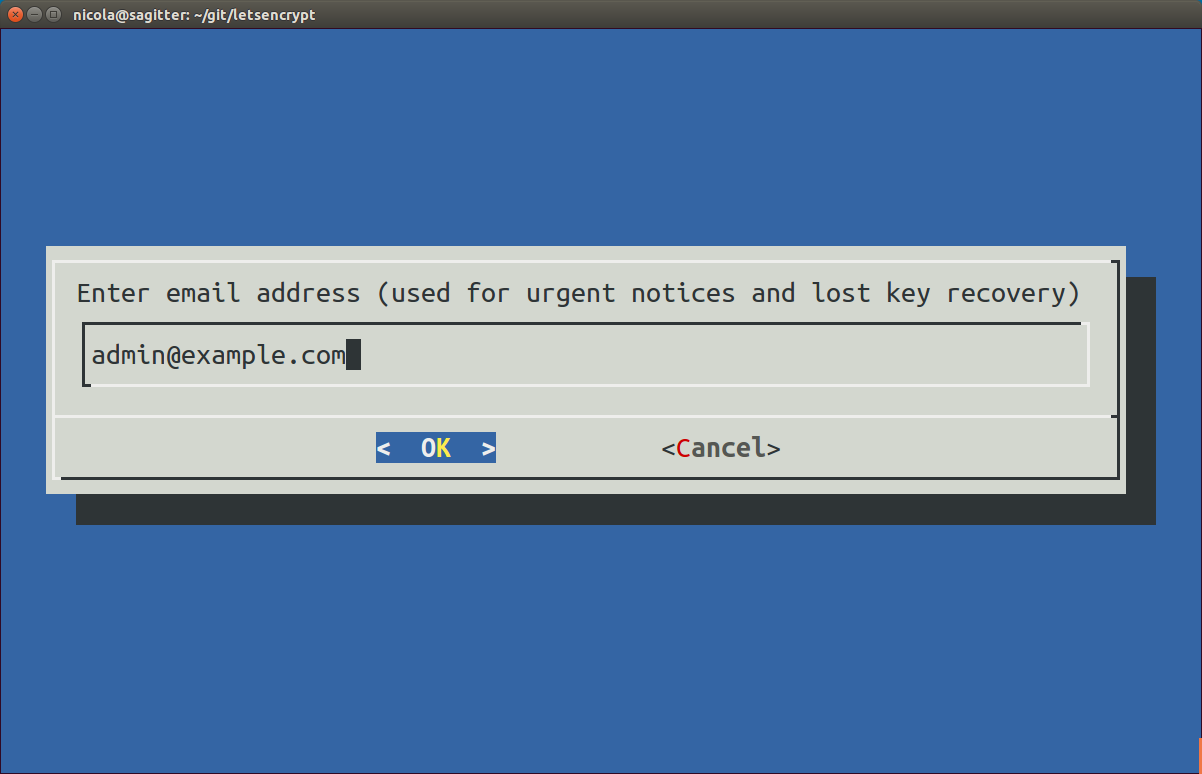
\includegraphics[width=9cm]{img/screen1.png}
\end{center}
\end{frame}
\begin{frame}{Screens}
\begin{center}
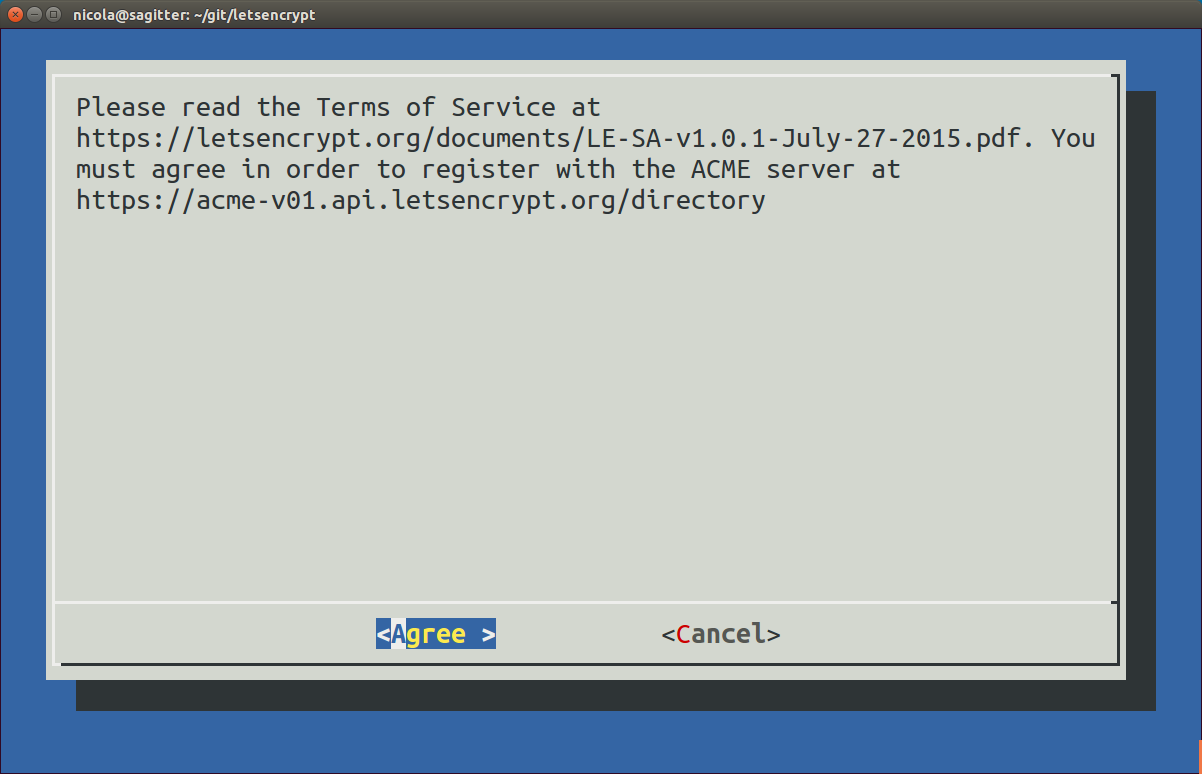
\includegraphics[width=9cm]{img/screen2.png}
\end{center}
\end{frame}
\begin{frame}{Screens}
\begin{center}
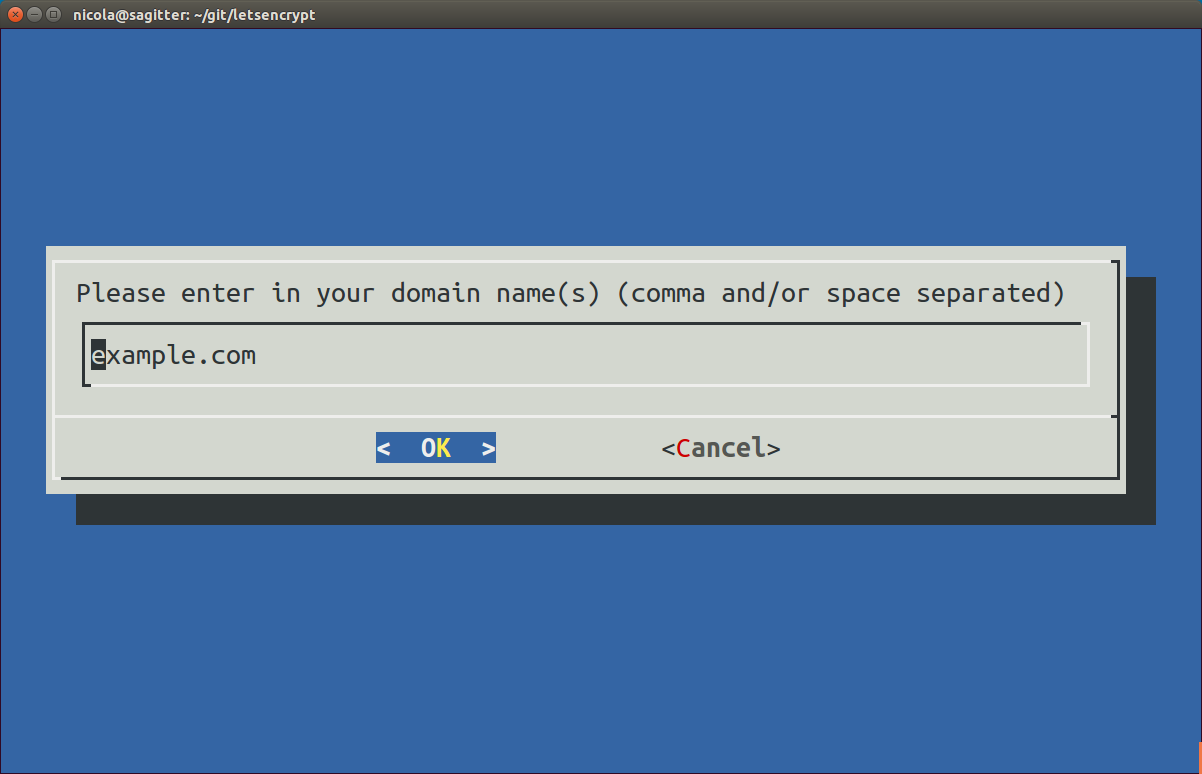
\includegraphics[width=9cm]{img/screen3.png}
\end{center}
\end{frame}
\begin{frame}{Screens}
\begin{center}
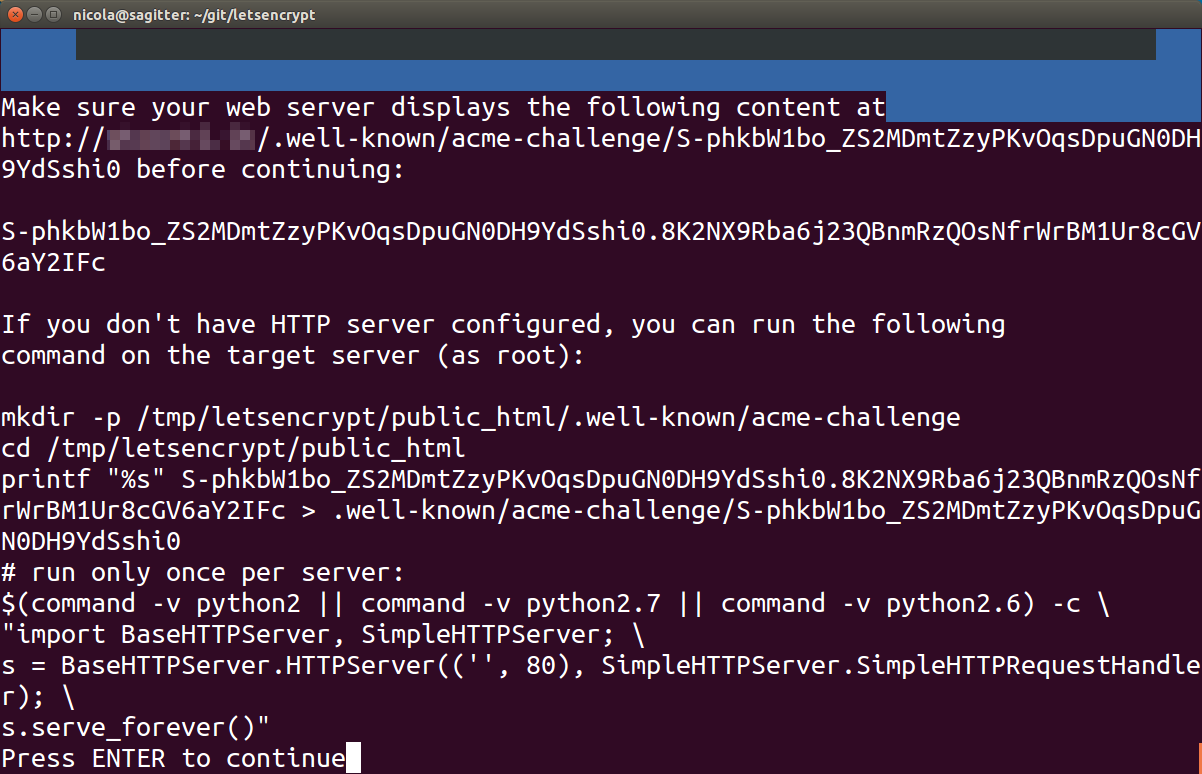
\includegraphics[width=9cm]{img/screen4.png}
\end{center}
\end{frame}
\begin{frame}{Screens}
\begin{center}
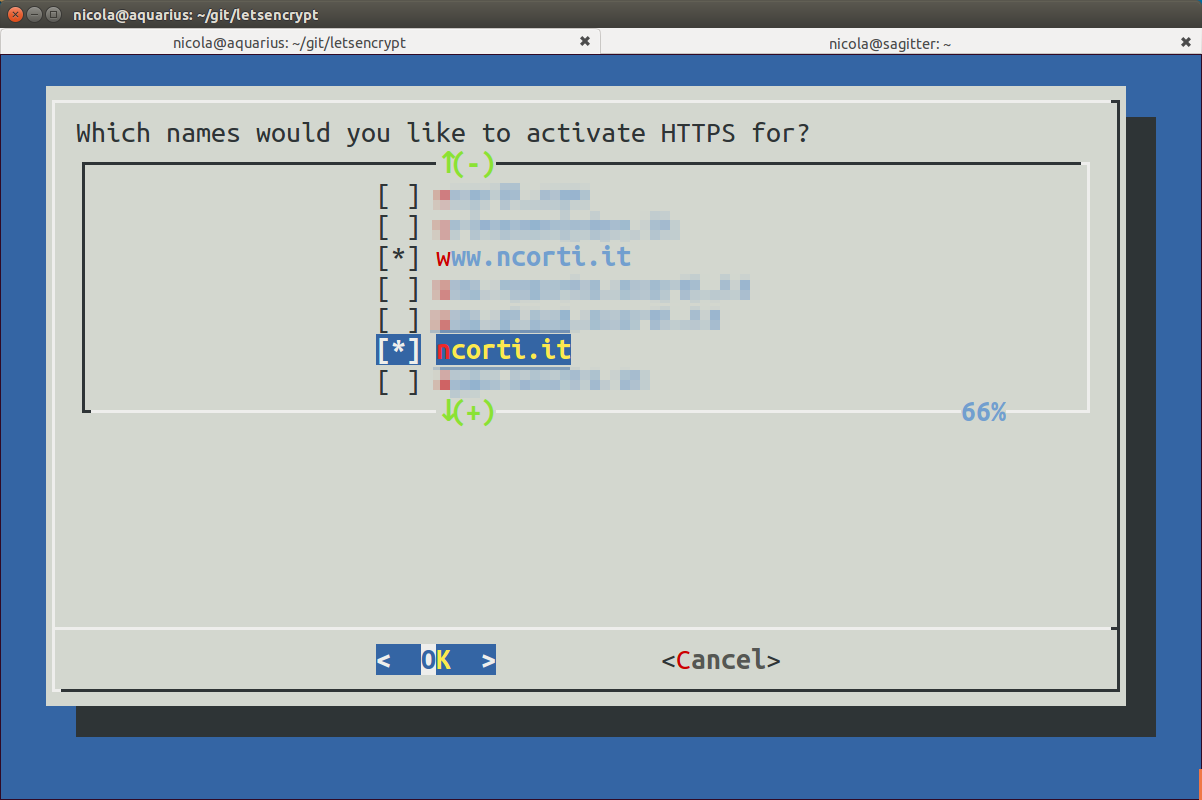
\includegraphics[width=9cm]{img/screen5.png}
\end{center}
\end{frame}
\begin{frame}{Screens}
\begin{center}
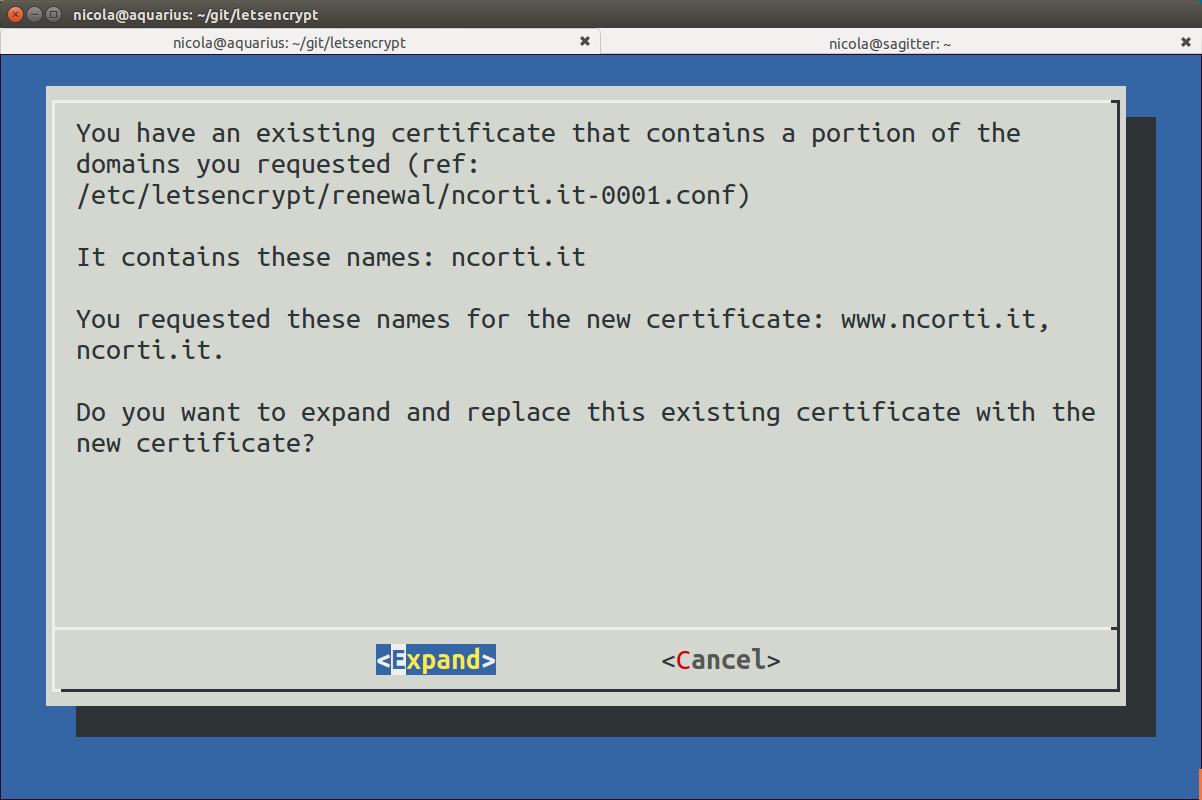
\includegraphics[width=9cm]{img/screen6.png}
\end{center}
\end{frame}
\begin{frame}{Screens}
\begin{center}
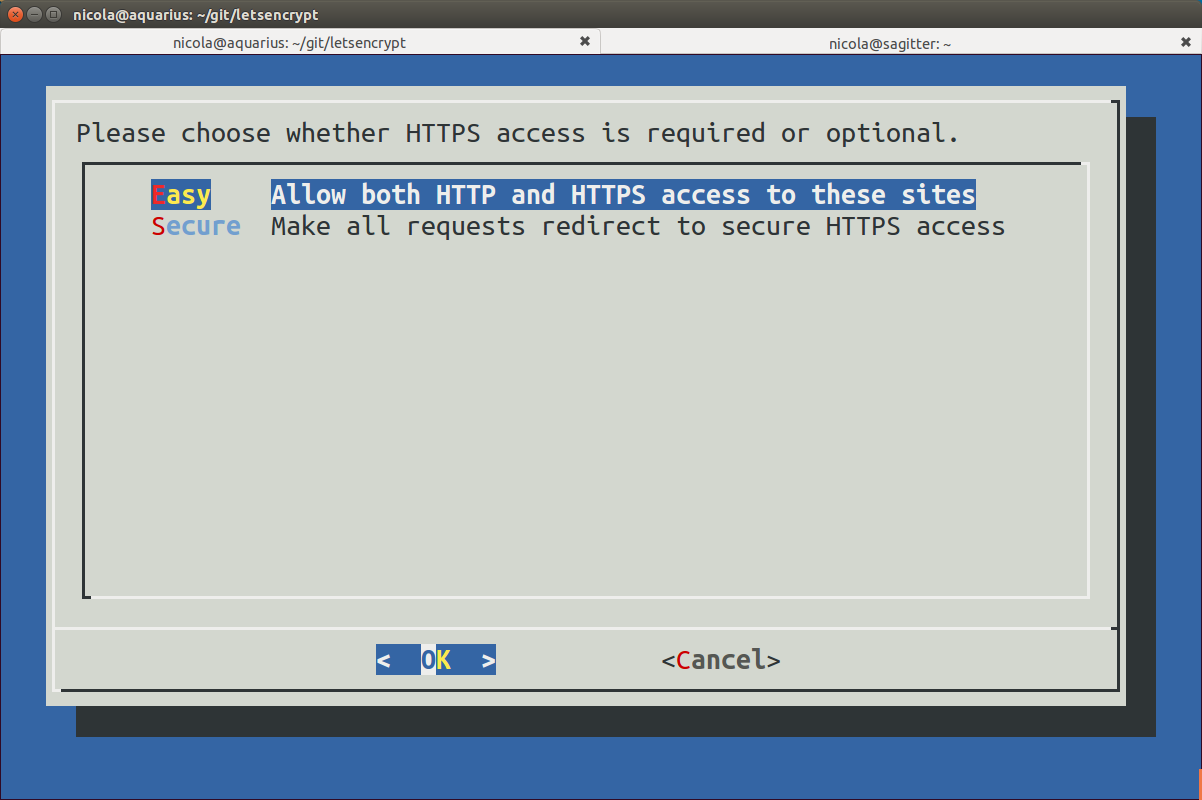
\includegraphics[width=9cm]{img/screen7.png}
\end{center}
\end{frame}
\begin{frame}{Screens}
\begin{center}
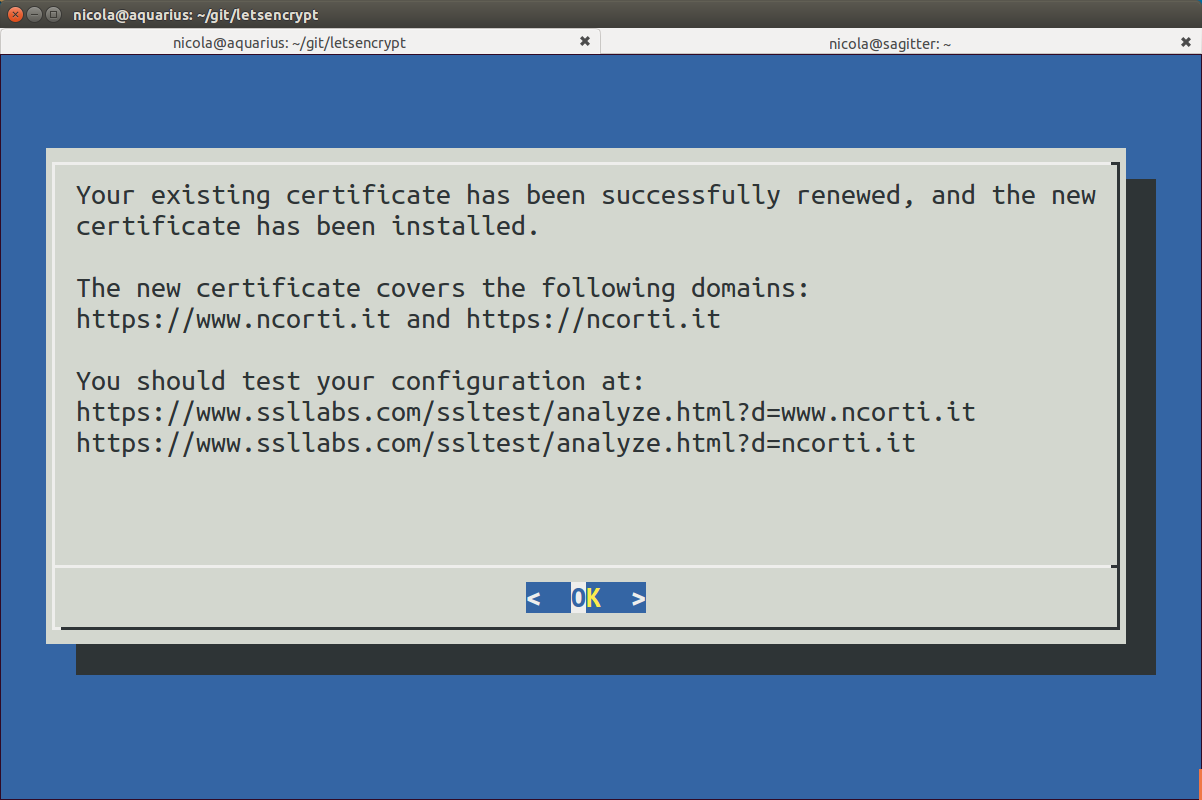
\includegraphics[width=9cm]{img/screen8.png}
\end{center}
\end{frame}


\section{Conclusions}
\begin{frame}{}
\begin{center}
\begin{Huge}
\textcolor{leorange}{\emph{Conclusions}}
\end{Huge}
\end{center}
\end{frame}



\subsection{Drawbacks}
\begin{frame}{Drawbacks}
\begin{itemize}
  \item No support for \textbf{Organization Validation} or \textbf{Extended Validation}, to hard to automate.
  \medskip\pause
  \item No support for \textbf{wildcards} (*.example.com), maybe in the future.
  \medskip\pause
  \item Only HTTP challenge is supported (public beta), DNS challenge support is not already available.
\end{itemize}
\end{frame}

\subsection{Resources}
\begin{frame}{Resources}
\begin{small}
\begin{itemize}
  \item How it works \textbf{\url{https://letsencrypt.org/howitworks/}}
  \medskip
  \item Tech details \textbf{\url{https://letsencrypt.org/howitworks/technology/}}
  \medskip
  \item Read the docs \textbf{\url{https://letsencrypt.readthedocs.org/}}
  \medskip
  \item Community board \textbf{\url{https://community.letsencrypt.org/}}
  \medskip
  \item Code \textbf{\url{https://github.com/letsencrypt/}}
  \medskip
  \item Mailing lists
  \begin{itemize}
    \item Client \textbf{\url{https://groups.google.com/a/letsencrypt.org/forum/\#!forum/client-dev}}
    \item Server \textbf{\url{https://groups.google.com/a/letsencrypt.org/forum/\#!forum/ca-dev}}
    \item ACME (IETF) \textbf{\url{https://www.ietf.org/mailman/listinfo/acme}}
  \end{itemize}
\end{itemize}
\end{small}
\end{frame}

\begin{frame}{}
\begin{center}
\begin{Huge}
{\color{leorange} \textbf{Questions...?}}
\end{Huge}

\vspace{1.5cm}
% \textbf{Nicola Corti - corti.nico [at] gmail [dot] com}\\

\begin{center}
\begin{tabular}{>{\centering\arraybackslash}p{4cm}}

\includegraphics[height=0.2cm]{img/logo_web.pdf} \textbf{\href{https://ncorti.com}{ ncorti.com}} \\

\includegraphics[height=0.2cm]{img/logo_twitter.pdf} \textbf{\href{https://twitter.com/cortinico}{ @cortinico}} \\

\includegraphics[height=0.2cm]{img/logo_gh.pdf} \textbf{\href{https://github.com/cortinico}{ @cortinico}} \\
\end{tabular}
\end{center}

\bigskip

\begin{footnotesize}
Made with \LaTeX\ Beamer.\\
This presentation is released under licence \\
\textbf{Creative Commons - Attributions, Non Commercial, Share-alike}.
\\
\medskip

\includegraphics[height=0.5cm]{img/cc.png}
\\
\medskip
Sources at \textbf{\url{https://github.com/cortinico/gulp-letsencrypt}}
\end{footnotesize}

\end{center}
\end{frame}

\end{document}
